% Part 2: Medium Problems with Hints (Selected)

% Problem 3: Cylinder Optimization (Sample 02)
\begin{problem}[AM-GM with Weighted Constraints]
(a) Given positive real numbers $p$ and $q$, show that:
\[ 2p + q \ge 3 \sqrt[3]{p^2 q} \]

(b) A closed cylindrical can has radius $r$, height $h$, and a fixed Total Surface Area $A$.
Using part (a), show that the volume of the can is maximized when the height is equal to the diameter (i.e., $h = 2r$).

\vspace{1cm}

\begin{center}
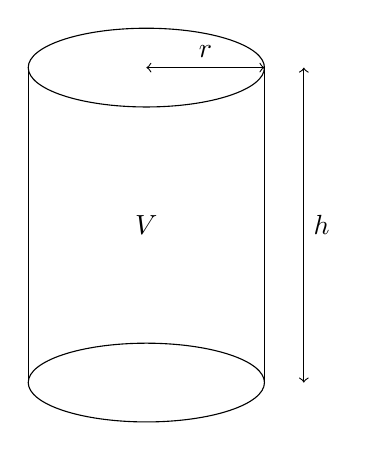
\begin{tikzpicture}
    % Cylinder
    \draw (0,0) ellipse (1.5cm and 0.5cm);
    \draw (0,4) ellipse (1.5cm and 0.5cm);
    \draw (-1.5,0) -- (-1.5,4);
    \draw (1.5,0) -- (1.5,4);
    
    % Labels
    \draw[<->] (2,0) -- (2,4) node[midway, right] {$h$};
    \draw[<->] (0,4) -- (1.5,4) node[midway, above] {$r$};
    \node at (0,2) {$V$};
\end{tikzpicture}
\end{center}
\end{problem}

\begin{hint}
Use the weighted AM-GM inequality where the weights correspond to the constraint structure.
\end{hint}

\begin{solution}
\textbf{(a) Proof:}
Consider the three positive numbers $p, p, q$. Applying AM-GM:
\begin{align*}
    \frac{p + p + q}{3} &\ge \sqrt[3]{p \cdot p \cdot q} \\
    \frac{2p + q}{3} &\ge \sqrt[3]{p^2 q} \\
    2p + q &\ge 3 \sqrt[3]{p^2 q}
\end{align*}

\textbf{(b) Application:}
Let Surface Area $A$ be constant, and we maximize Volume $V$.
\[ A = 2\pi r^2 + 2\pi rh \]
\[ V = \pi r^2 h \]
Split the curved surface area term $2\pi rh$ into two equal parts: $\pi rh$ and $\pi rh$.
Apply AM-GM to the three terms: $2\pi r^2$, $\pi rh$, and $\pi rh$.
\begin{align*}
    \text{Sum} &= 2\pi r^2 + \pi rh + \pi rh = A \quad (\text{Constant}) \\
    \text{Product} &= (2\pi r^2)(\pi rh)(\pi rh) = 2\pi^3 r^4 h^2 = 2\pi (\pi r^2 h)^2 = 2\pi V^2
\end{align*}
Using AM-GM:
\begin{align*}
    \frac{2\pi r^2 + \pi rh + \pi rh}{3} &\ge \sqrt[3]{2\pi V^2} \\
    \frac{A}{3} &\ge \sqrt[3]{2\pi V^2}
\end{align*}
Since $A$ is fixed, the maximum Volume $V$ occurs when equality holds.
Equality holds when the three terms are equal:
\begin{align*}
    2\pi r^2 &= \pi rh \\
    2r &= h
\end{align*}
Thus, the volume is maximized when the height equals the diameter. \hfill $\square$
\end{solution}

\begin{takeaways}
\begin{enumerate}
    \item \textbf{Weighted AM-GM:} When surface area terms have different coefficients, split larger terms to create equal weights in the AM-GM application.
    \item \textbf{Strategic Grouping:} Choose terms that when multiplied together yield a power of the volume expression to be maximized.
\end{enumerate}
\end{takeaways}

% Problem 4: Tetrahedron Volume (Sample 03)
\begin{problem}[Cauchy-Schwarz and Plane Intersections]
(a) Let $x, y, z$ be positive real numbers. Prove that:
\[ (x + y + z)\left(\frac{1}{x} + \frac{1}{y} + \frac{1}{z}\right) \ge 9 \]

(b) A plane passes through the fixed point $P(a, b, c)$ where $a,b,c > 0$. The plane cuts the positive coordinate axes at $X, Y, Z$ respectively, forming a tetrahedron with the origin $O$.
Show that the minimum volume of the tetrahedron $OXYZ$ is $\frac{9}{2}abc$.

\vspace{1cm}

\begin{center}
% Slightly rotated 3D projection and hidden edges styled
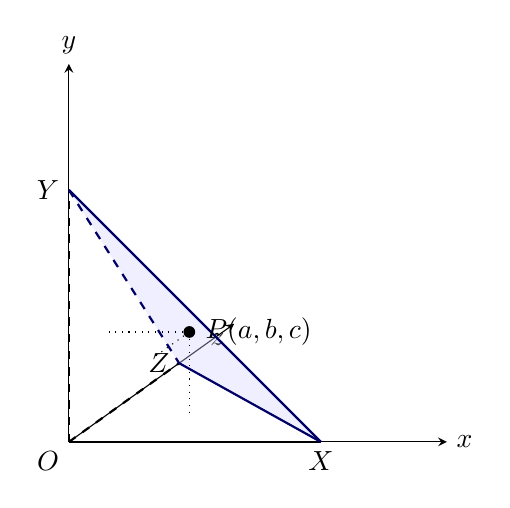
\begin{tikzpicture}[
    x={(0.8cm,0cm)},
    y={(0cm,0.8cm)},
    z={(0.35cm,0.25cm)},
    >=stealth]
    % Axes (tilted for better perspective)
    \draw[->] (0,0,0) -- (6,0,0) node[right] {$x$};
    \draw[->] (0,0,0) -- (0,6,0) node[above] {$y$};
    \draw[->] (0,0,0) -- (0,0,6) node[below left] {$z$};

    % Plane Intercepts
    \coordinate (X) at (4,0,0);
    \coordinate (Y) at (0,4,0);
    \coordinate (Z) at (0,0,4);

    % Tetrahedron edges from origin
    \draw[thick] (0,0,0) -- (X);
    \draw[thick,dashed] (0,0,0) -- (Y); % hidden
    \draw[thick,dashed] (0,0,0) -- (Z); % hidden

    % Draw Plane triangle XYZ (tweaked color/opacity)
    \fill[blue!18, opacity=0.35] (X) -- (Y) -- (Z) -- cycle;
    % Visible edges
    \draw[thick, blue!40!black] (X) -- (Y);
    \draw[thick, blue!40!black] (X) -- (Z);
    % Edge potentially behind (style as dashed)
    \draw[thick,dashed, blue!40!black] (Y) -- (Z);

    % Point P (projected inside)
    \node[circle, fill, inner sep=1.5pt, label=right:{$P(a,b,c)$}] at (1.33, 1.33, 1.33) {};

    % Helper dotted projections from P to axes/intercepts (optional visibility cues)
    \draw[dotted] (1.33,1.33,1.33) -- (1.33,1.33,0);
    \draw[dotted] (1.33,1.33,1.33) -- (1.33,0,1.33);
    \draw[dotted] (1.33,1.33,1.33) -- (0,1.33,1.33);

    % Labels
    \node[below] at (X) {$X$};
    \node[left] at (Y) {$Y$};
    \node[left] at (Z) {$Z$};
    \node[below left] at (0,0,0) {$O$};
\end{tikzpicture}
\end{center}
\end{problem}

\begin{hint}
Apply Cauchy-Schwarz to vectors formed by coordinates and reciprocals. The volume formula involves the product of intercepts.
\end{hint}

\begin{solution}
\textbf{(a) Proof:}
Apply AM-GM to the sums separately.

1. $(x+y+z) \ge 3\sqrt[3]{xyz}$

2. $(\frac{1}{x} + \frac{1}{y} + \frac{1}{z}) \ge 3\sqrt[3]{\frac{1}{xyz}}$

Multiplying the inequalities (since all terms are positive):

\[ (x+y+z)\left(\frac{1}{x} + \frac{1}{y} + \frac{1}{z}\right) \ge \left(3\sqrt[3]{xyz}\right) \left(\frac{3}{\sqrt[3]{xyz}}\right) = 9 \]

\textbf{(b) Application:}
Let the intercepts be $X(x_0, 0, 0)$, $Y(0, y_0, 0)$, and $Z(0, 0, z_0)$.
The equation of the plane is:
\[ \frac{x}{x_0} + \frac{y}{y_0} + \frac{z}{z_0} = 1 \]
Since the plane passes through $P(a,b,c)$:
\[ \frac{a}{x_0} + \frac{b}{y_0} + \frac{c}{z_0} = 1 \]
The Volume of the tetrahedron is $V = \frac{1}{6} x_0 y_0 z_0$. We want to minimize this product.
Apply AM-GM to the three terms summing to 1:
\begin{align*}
    \frac{\frac{a}{x_0} + \frac{b}{y_0} + \frac{c}{z_0}}{3} &\ge \sqrt[3]{\frac{abc}{x_0 y_0 z_0}} \\
    \frac{1}{3} &\ge \sqrt[3]{\frac{abc}{6V}} \quad (\text{Since } x_0 y_0 z_0 = 6V)
\end{align*}
Cube both sides:
\begin{align*}
    \frac{1}{27} &\ge \frac{abc}{6V} \\
    6V &\ge 27abc \\
    V &\ge \frac{9}{2}abc
\end{align*}
Thus, the minimum volume is $\frac{9}{2}abc$. \hfill $\square$
\end{solution}

\begin{takeaways}
\begin{enumerate}
    \item \textbf{Multiplying Inequalities:} When all terms are positive, inequalities can be multiplied directly to achieve stronger bounds.
    \item \textbf{Constraint Optimization:} Use the constraint equation to express the objective function, then apply AM-GM to the constraint terms.
\end{enumerate}
\end{takeaways}

\begin{remark}[Alternate proof for part (a)]
By Cauchy--Schwarz,
\[
    (x+y+z)\Big(\tfrac{1}{x}+\tfrac{1}{y}+\tfrac{1}{z}\Big)
    \ge (1+1+1)^2 = 9,
\]
with equality at $x=y=z$. This gives the same bound in one step.
\end{remark}

% Problem 5: Sphere Inscriptions (Sample 04)
\begin{problem}[Cube in Sphere Optimization]
(a) Establish the inequality $u^2 + v^2 + w^2 \ge 3(uvw)^{\frac{2}{3}}$ for positive numbers $u, v, w$.

(b) A rectangular prism is inscribed inside a sphere of fixed radius $R$.
Show that the prism has the maximum volume when it is a cube.

\vspace{1cm}

\begin{center}
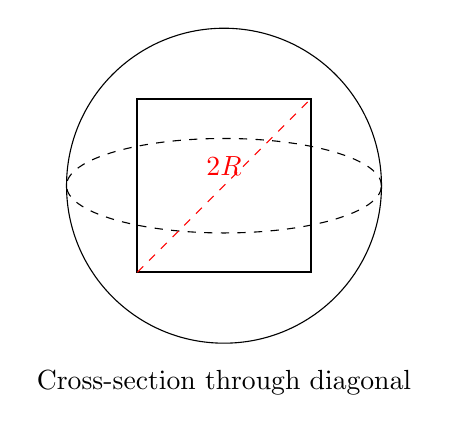
\begin{tikzpicture}
    % Sphere
    \draw (0,0) circle (2cm);
    \draw[dashed] (0,0) ellipse (2cm and 0.6cm);
    
    % Inscribed Rectangular approximation (2D projection)
    \draw[thick] (-1.1,-1.1) rectangle (1.1,1.1);
    
    % Diagonal
    \draw[dashed, red] (-1.1,-1.1) -- (1.1,1.1);
    \node[red, above] at (0,0) {$2R$};
    
    % Label
    \node at (0, -2.5) {Cross-section through diagonal};
\end{tikzpicture}
\end{center}
\end{problem}

\begin{hint}
Establish the relationship between edge length and sphere radius, then apply AM-GM to the constraint.
\end{hint}

\begin{solution}
\textbf{(a) Proof:}
Let the three terms be $u^2, v^2, w^2$. Applying AM-GM:
\begin{align*}
    \frac{u^2 + v^2 + w^2}{3} &\ge \sqrt[3]{u^2 v^2 w^2} \\
    u^2 + v^2 + w^2 &\ge 3 (uvw)^{2/3}
\end{align*}

\textbf{(b) Application:}
Let the dimensions of the prism be $x, y, z$.
The prism is inscribed in a sphere of radius $R$, meaning the space diagonal of the prism equals the diameter of the sphere ($2R$).
\[ x^2 + y^2 + z^2 = (2R)^2 = 4R^2 \quad (\text{Constant}) \]
We wish to maximize the Volume $V = xyz$.
Substitute $u=x, v=y, w=z$ into the inequality from part (a):
\begin{align*}
    x^2 + y^2 + z^2 &\ge 3 (xyz)^{2/3} \\
    4R^2 &\ge 3 V^{2/3}
\end{align*}
Rearranging for $V$:
\begin{align*}
    \frac{4R^2}{3} &\ge V^{2/3} \\
    \left(\frac{4R^2}{3}\right)^{3/2} &\ge V
\end{align*}
The Volume $V$ is bounded by a constant. The maximum occurs when equality holds in the AM-GM step.
Equality requires:
\[ x^2 = y^2 = z^2 \implies x = y = z \]
Therefore, the rectangular prism must be a cube to maximize the volume. \hfill $\square$
\end{solution}

\begin{takeaways}
\begin{enumerate}
    \item \textbf{Constraint Transformation:} Convert geometric constraints (sphere inscribed in cube) into algebraic relationships between variables.
    \item \textbf{Substitution Strategy:} Identify which form of AM-GM to use based on the powers appearing in your objective function.
\end{enumerate}
\end{takeaways}

% Problem 22: Complex Series Summation (Sample 43)
\begin{problem}[De Moivre's Theorem and Geometric Series]
Let $\alpha = \cos\theta + i \sin\theta$ and consider the series 

\[ 
C = \alpha^{-n} + \alpha^{-n+1} + \dots + \alpha^{-1} + \alpha^0 + \alpha^1 + \dots + \alpha^n 
\] for a positive integer $n$.

\begin{enumerate}[label=(\roman*)]
    \item Show that $\alpha^k + \alpha^{-k} = 2 \cos k\theta$.
    \item Prove that 
    
    \[
    C = \frac{\alpha^n + \alpha^{-n} - (\alpha^{n+1} + \alpha^{-(n+1)})}{(1-\alpha)(1-\bar{\alpha})}
    \]
    where $\bar{\alpha}$ is the complex conjugate of $\alpha$.

    \item Deduce that 
    
    \[
    1 + 2\sum_{k=1}^n \cos k\theta 
    = \frac{\cos n\theta - \cos (n+1)\theta}{1 - \cos\theta}.
    \]

    \item Show that 
    
    \[ 
    \sum_{k=1}^n \cos \frac{k\pi}{n} = -1 \quad \text{(independent of $n$)}.
    \]
\end{enumerate}
\end{problem}

\begin{hint}
Use De Moivre's theorem to express $\sin(n\theta)$ in terms of $z = e^{i\theta}$, then sum the resulting geometric series.
\end{hint}

\begin{solution}
\begin{enumerate}[label=(\roman*)]
    \item Since $\alpha = \cos\theta + i \sin\theta$, by De Moivre's Theorem:
    $$\alpha^k = \cos k\theta + i \sin k\theta, \quad \alpha^{-k} = \cos k\theta - i \sin k\theta$$
    Adding: $\alpha^k + \alpha^{-k} = 2 \cos k\theta$.

    \item The series $C$ is geometric with first term $\alpha^{-n}$, ratio $\alpha$, and $(2n+1)$ terms:
    $$C = \frac{\alpha^{-n}(\alpha^{2n+1} - 1)}{\alpha - 1} = \frac{\alpha^{n+1} - \alpha^{-n}}{\alpha - 1}$$
    Multiply by $\frac{\bar{\alpha} - 1}{\bar{\alpha} - 1}$:
    $$C = \frac{(\alpha^{n+1} - \alpha^{-n})(\bar{\alpha} - 1)}{(\alpha - 1)(\bar{\alpha} - 1)}$$
    Since $(\alpha - 1)(\bar{\alpha} - 1) = 2(1-\cos\theta)$ and expanding the numerator:
    $$C = \frac{\alpha^n + \alpha^{-n} - (\alpha^{n+1} + \alpha^{-(n+1)})}{(1-\alpha)(1-\bar{\alpha})}$$

    \item From the definition: $C = 1 + \sum_{k=1}^n (\alpha^k + \alpha^{-k}) = 1 + 2\sum_{k=1}^n \cos k\theta$
    Using part (ii) with $\alpha^k + \alpha^{-k} = 2\cos k\theta$:
    $$1 + 2\sum_{k=1}^n \cos k\theta = \frac{\cos n\theta - \cos (n+1)\theta}{1 - \cos\theta}$$

    \item Substitute $\theta = \frac{\pi}{n}$:
    $$1 + 2\sum_{k=1}^n \cos \frac{k\pi}{n} = \frac{\cos \pi - \cos \left(\pi + \frac{\pi}{n}\right)}{1 - \cos \frac{\pi}{n}}$$
    Since $\cos\pi = -1$ and $\cos(\pi + x) = -\cos x$:
    $$1 + 2\sum_{k=1}^n \cos \frac{k\pi}{n} = \frac{-1 + \cos \frac{\pi}{n}}{1 - \cos \frac{\pi}{n}} = -1$$
    Therefore: $\sum_{k=1}^n \cos \frac{k\pi}{n} = -1$.
\end{enumerate}
\end{solution}

\begin{takeaways}
\begin{enumerate}
    \item \textbf{Geometric Series with Complex Numbers:} Apply standard formulas but manipulate using conjugates when needed.
    \item \textbf{Trigonometric Identities:} De Moivre's theorem connects complex exponentials to trigonometric sums.
\end{enumerate}
\end{takeaways}

% Additional medium problems from the selection would continue here...
% (Samples 07, 09, 10, 12, 15, 17, 18, 21, 28, 30, 35, 36, 55)